%!TEX root = ../main.tex
% !TeX spellcheck = en_GB 
\chapter{Evaluation}%-----------------------------------------------------------
\label{sec:overtaking-and-head-on}
Four scenarios are defined in order to test the ANS in multi vessel situations. However, a simple crossing scenario is first shown to test the algorithm in a basic COLREGs situation. Ideas for the other scenarios are from \textcite{ecolreg_overtaking-and-crossing-2,ecolreg_overtaking-and-crossing-3,ecolreg_overtaking-and-crossing,ecolreg_overtaking-and-head-on}, with a few minor modifications. All scenarios are set in high visibility on the high sea.

\section{Crossing scenario}%-----------------------------------------

\begin{figure}[h]
    \centering
    \includegraphics[width=\textwidth,height=0.75\textheight,keepaspectratio]{Figures/Scenario/simple-scen.pdf}
    \caption{Crossing scenario}
    \label{fig:simple-scen}
\end{figure}

The first scenario depicts a simple crossing situation where two vessels are on perpendicular courses. The vessels start at perpendicular courses approximately 14 NM from each other with a speed of 10 kts as seen in figure \ref{fig:simple-scen}. The vessels max speed is set to 12 kts and maximum rate of turn 3 \textdegree /s. The two vessels collide in origo if no corrections are made to either course or speed. COLREGs \textit{rule 15} stipulate that vessel (\textit{A}) that has the other vessel on its starboard side  in a crossing situation should alter its course to starboard and avoid passing in front of the other vessel (\textit{B}).
\begin{figure}[h]
    \centering
    \includegraphics[width=\textwidth,height=0.75\textheight,keepaspectratio]{Figures/Scenario/simple-scen-res.pdf}
    \caption{Crossing scenario}
    \label{fig:simple-scen-res}
\end{figure}

Figure \ref{fig:simple-scen-res} shows the scenario when both boats are guided by the FIS system. The numbers on the vessels tracks are printed every thousand second, which equal 16 minutes and 40 seconds, and help to compare the vessels positions at a given time frame. These numbers will from here on be referred to with bold numbers. It can be seen that both vessels continue along their original paths until vessel \textit{A} reaches \textbf{1}, at which point the distance to vessel \textit{B} has shrunken to 10NM and the algorithm becomes aware of the target vessel. Vessel \textit{A} will at this point initiate a starboard turn to pass behind vessel \textit{C} as specified in COLREGs. Vessel \textit{A} will then continue on the heading suggested by the FIS until almost at \textbf{3} where  vessel \textit{B} is no longer considered a threat, i.e. no rule in the FIS applies, after which it steers back to its original heading.

The colours of the vessels paths shows their speed at that instance. Grey is equal to the original speed. A red tint means a speed above the original and a blue tint below. The stronger the tint, the higher the difference. It is worth noticing that vessel \textit{B} increases it speed slightly before  \textbf{3} since one of the rules states so, even though there is no collision risk.
\todo{explain why this happens}
\section{Overtaking and head-on scenario}%-----------------------------------------
\begin{figure}[h]
    \centering
    \includegraphics[width=\textwidth,height=0.75\textheight,keepaspectratio]{Figures/Scenario/overtaking-and-head-on.pdf}
    \caption{Overtaking and head-on scenario  \cite{ecolreg_overtaking-and-head-on}}
    \label{fig:overtaking-and-head-on}
\end{figure}
This scenario defines a three vessel scenario, where two vessels are meeting on a reciprocal courses. One of the vessels is, furthermore, overtaking a third vessel on the stand on vessels starboard side. A visualization of the scenario is shown in figure \ref{fig:overtaking-and-head-on}. Vessels \textit{A} and \textit{B} starts on reciprocal tracks 20 NM from each other, while \textit{B} and \textit{C} starts abreast 5 NM from each other. \textit{A}, \textit{B}, and \textit{C} has an max speed of 15 kts. \textit{A} and \textit{B} starts at 12 kts while \textit{C} is slightly slower at 10 kts. Max rate of turn of all vessels is set to 3\textdegree/second.

Vessels \textit{A} and \textit{B} are therefore obliged to alter their courses to starboard to prevent a head on collision (\textit{Rule 14}). Moreover vessel \textit{B} shall keep out of the way of \textit{C}  and in no circumstance alter its course so that it becomes a crossing vessel to \textit{C} (\textit{Rule 13}). All corrections shall furthermore be ample, so that it is recognizable by the other vessel, and taken as early as possible (\textit{Rule 16}) \cite{ecolreg_overtaking-and-head-on}.

\textcite{ecolreg_overtaking-and-head-on} suggest that vessel \textit{A} should alter course to starboard and pass ahead of vessel C,  to avoid collision.

\begin{figure}[h]
    \centering
    \includegraphics[width=\textwidth,height=0.75\textheight,keepaspectratio]{Figures/Scenario/overtaking-and-head-on-res.pdf}
    \caption{Overtaking and head-on scenario  }
    \label{fig:overtaking-and-head-on-res}
\end{figure}

\todo{Evaluate result}
\section{Overtaking and crossing scenario 1}%---------------------------------------
\label{sec:overtaking-and-crossing}
\begin{figure}[h]
    \centering
    \includegraphics[width=\textwidth,height=0.75\textheight,keepaspectratio]{Figures/Scenario/overtaking-and-crossing.pdf}
    \caption{Overtaking and crossing scenario 1 \cite{ecolreg_overtaking-and-crossing}}
    \label{fig:overtaking-and-crossing}
\end{figure}
The following three scenarios both depict scenario where vessels \textit{A} and \textit{B} is in an overtaking situation while \textit{C} crosses both their paths. \textit{C} crosses \textit{A} and \textit{B}s paths with a 45\textdegree  angle in the first scenario (figure \ref{fig:overtaking-and-crossing}). \textit{A} starts at (-5, -6), \textit{B} at (0, -9) and \textit{C} in (9,8). \textit{A} and \textit{B} has an initial heading of 0\textdegree  while \textit{C} start with a heading of 235\textdegree. The speeds of the vessels is set to ensure that \textit{C} will collide with both vessels if no corrections are applied. Moreover the speed of \textit{B} must be greater than the speed of \textit{A} since \textit{B} is overtaking \textit{A}. The vessels initial speed are, therefore: \textit{A} = 2kts, \textit{B} = 7kts and \textit{C} = 7.6kts. The maximum speeds of the vessels are 10, 15 and 20 kts respectively. Max rate of turn of all vessels is set to 3\textdegree/second.

Rule 13 and 16 applies to this scenario in the same way as the previous one, with the exception that the vessels involved in the overtaking situation is vessel \textit{A} and \textit{B} instead of \textit{B} and \textit{C}. This implies that \textit{B} shall keep out of way of \textit{A} (\textit{Rule 13}), while \textit{A} shall keep its course and speed (\textit{Rule 17}).

Additionally both \textit{A} and \textit{B} are crossing \textit{C}s path with a risk of collision. This means that \textit{A} and \textit{B} should alter their courses to starboard and avoid passing in front of \textit{C} (\textit{Rule 15}). Vessel \textit{C} shall, meanwhile, keep its course and speed. This results in contradictory obligations for vessel  \textit{A}, where it should keep its course and speed for \textit{B} and simultaneously keep out of the way for vessel \textit{C}.

\textcite{ecolreg_overtaking-and-crossing} suggest the following manoeuvres for vessel \textit{A} and \textit{B} in accordance with the ordinary practice of seamen:
Both vessels might alter course to starboard and, thereby, pass behind vessel \textit{C}. Alternatively vessel \textit{A} may reduce speed or make a 360\textdegree turn to port, while vessel \textit{B} reduces speed, makes a 360\textdegree to starboard or alters its course to starboard.

\begin{figure}[h]
    \centering
    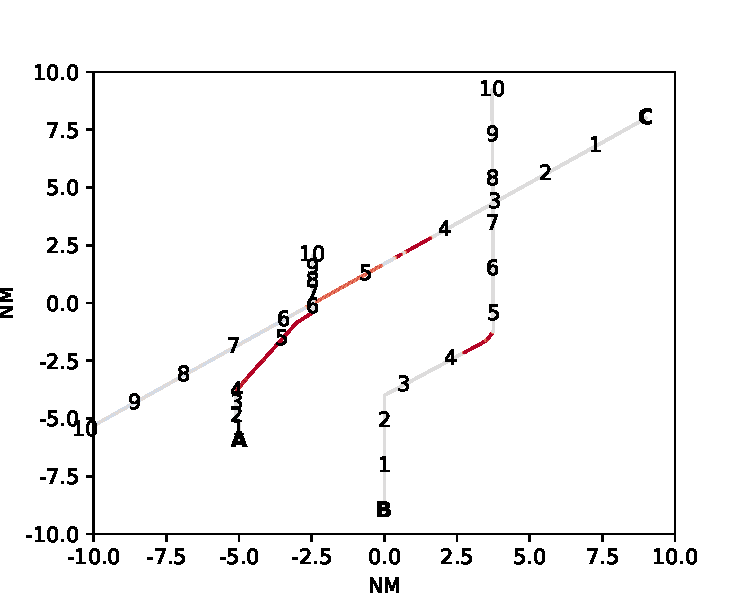
\includegraphics[width=\textwidth,height=0.75\textheight,keepaspectratio]{Figures/Scenario/overtaking-and-crossing-res.pdf}
    \caption{Overtaking and crossing scenario 1}
    \label{fig:overtaking-and-crossing-res}
\end{figure}
\todo{Evaluate result}
\section{Overtaking and crossing scenario 2}%---------------------------------------

\begin{figure}[h]
    \centering
    \includegraphics[width=\textwidth,height=0.75\textheight,keepaspectratio]{Figures/Scenario/overtaking-and-crossing-3.pdf}
    \caption{Overtaking and crossing scenario 2 \cite{ecolreg_overtaking-and-crossing-3}}
    \label{fig:overtaking-and-crossing-3}
\end{figure}
The next scenario, visualized in figure \ref{fig:overtaking-and-crossing-3}, differs from the previous only in that B and C are not in risk of collission since Bs speed is decreased to 4 kts. This means that B has no obligations to alter its course to starboard to avoid C as in the previous sceanrio. All other rules from the previous scenario does apply and vessel A is, therefore, still in the contradictory situation where it shall both keep course and speed for vessel B and alter course to starboard to avoid vessel C.

The following actions by vessel A solves the situation in accordance with the ordinary practice of seamen. It might either slow down, make a 360 degree turn to port or alter course to starboard and pass in front of vessel B if time permits.



\begin{figure}[h]
    \centering
    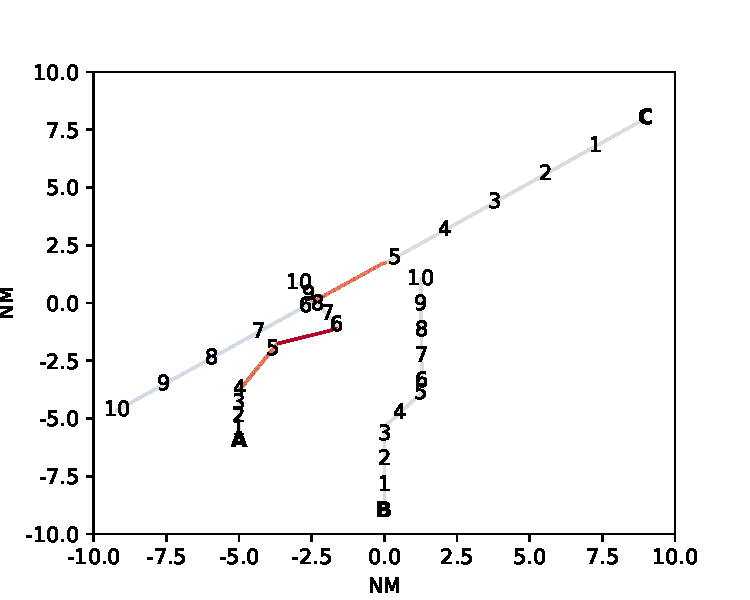
\includegraphics[width=\textwidth,height=0.75\textheight,keepaspectratio]{Figures/Scenario/overtaking-and-crossing-3-res.pdf}
    \caption{Overtaking and crossing scenario 2}
    \label{fig:overtaking-and-crossing-3-res}
\end{figure}
\todo{Evaluate result}
\section{Overtaking and crossing scenario 3}%---------------------------------------

\begin{figure}[h]
    \centering
    \includegraphics[width=\textwidth,height=0.75\textheight,keepaspectratio]{Figures/Scenario/overtaking-and-crossing-2.pdf}
    \caption{Overtaking and crossing scenario 3 \cite{ecolreg_overtaking-and-crossing-2}}
    \label{fig:overtaking-and-crossing-2}
\end{figure}

The last scenario depicts a similar scenario as the previous two, with two vessels in an overtaking situation while a third crosses their paths. The scenario is visualized in figure \ref{fig:overtaking-and-crossing-2}. Vessel \textit{A} starts at (0,-10), vessel \textit{B} at (3.6, 5) and \textit{C} at (10,0). The two vessels involved in the overtaking situation, that is \textit{A} and \textit{B}, starts with a heading of 0 \textdegree while  \textit{C} starts with a 270 \textdegree heading in order to cross the two other vessels paths perpendicularly. \textit{A} and \textit{C} start at a speed of 10 kts while \textit{B} starts at 15 kts. All vessels has as maximum speed of 20 kts and a maximum rate of turn of 3 \textdegree /s. The same rules apply as in the two previous rules, but the manoeuvring space for vessels \textit{A} and \textit{B} is slightly more limited due to the angle which C approaches on.

Vessel \textit{A} is also in this scenario in a situation where two rules contradict each other.
It shall keeps course and speed for vessel \textit{B} while simultaneously avoiding vessel \textit{C}.
Vessel \textit{C} shall keep course and speed for both vessel \textit{B} and \textit{A}.
Finally vessel \textit{B} shall keep out of the way of vessel \textit{A} and alter course to starboard to avoid vessel C.

One of the following actions is recommended to avoid collisions \cite{ecolreg_overtaking-and-crossing-2}. Both vessels might alter their course to starboard and pass behind vessel \textit{C} to avoid collision. The action must however be initiated by vessel \textit{B}. Alternatively vessel \textit{A} might either reduce speed or make a 360 degree turn. The turn must be initiated early if made to starboard. Vessel \textit{B} must at the same time also reduce speed, make a 360 \textdegree turn to starboard or alter course to starboard to avoid colliding with vessel \textit{C}



\begin{figure}[h]
    \centering
    \includegraphics[width=\textwidth,height=0.75\textheight,keepaspectratio]{Figures/Scenario/overtaking-and-crossing-2-res.pdf}
    \caption{Overtaking and crossing scenario 3}
    \label{fig:overtaking-and-crossing-2-res}
\end{figure}
\todo{Evaluate result}
%------------------------------------------------------------------------------------

\chapter{Discussion}
\label{chap:disc}
%ändta range params för olika situationer
% Sometimes correctionts even though the vessels are not on collision course
\chapter{Conclusion}